% \documentclass{article}
\documentclass[journal=jpclcd,manuscript=article]{achemso}
\usepackage[utf8]{inputenc}

% ALL: See "style guide" here: % https://docs.google.com/document/d/12xwId6RT73miifI1thtLL7c0GoVIXsSfZndO5bgdqag/edit#

% Tables
% Use Roman numerals for tables
% https://tex.stackexchange.com/a/226029
\usepackage[labelsep=period]{caption}
\captionsetup[table]{name=Table}
\renewcommand{\thefigure}{S\arabic{figure}}
\renewcommand{\thetable}{S\Roman{table}}
% \usepackage{multirow}

\usepackage{pdflscape}
\usepackage{textcomp}
\usepackage{gensymb}
\usepackage{geometry}
\usepackage{multirow}

\usepackage{subcaption} % For subfigures?

\usepackage{pifont}
\newcommand{\cmark}{\textcolor{blue}{\textrm{\ding{52}}}}%
\newcommand{\xmark}{\textcolor{red}{\textrm{\ding{56}}}}%

\usepackage{amsmath}
\usepackage{amssymb}
%usepackage{authblk}


% units
% \SI{X}{\UNIT} will write the value X with units \UNIT. 
% eg. \SI{30}{\celsius}
\usepackage{siunitx} 

\usepackage{graphicx}
\graphicspath{ {./images/} }

\setlength {\marginparwidth }{2cm}
\usepackage{todonotes}
\newcommand{\tino}[1]{\todo[inline,color=purple!40]{Tino: #1}}
\newcommand{\fbp}[1]{\todo[inline,color=orange!40]{Ferran: #1}}
\newcommand{\summary}[1]{\todo[inline,caption={},color=yellow!40]{Summary: \\ #1}}

\newcommand{\ssri}[1]{{
\fbox{
\parbox{0.8\textwidth}{  \fbox{$\triangleright$\textcolor{blue}{\textbf{Shashank}:}} 
#1
}}}}

\newcommand{\gbox}[1]{{
\fbox{
\parbox{0.8\textwidth}{  \fbox{$\triangleright$\textcolor{blue}{\textbf{Gon}:}} 
#1
}}}}

\newcommand{\pbox}[1]{{
\fbox{
\parbox{0.8\textwidth}{  \fbox{$\triangleright$\textcolor{blue}{\textbf{From Peter}:}} 
#1
}}}}

\newcommand{\pdebox}[1]{{
\fbox{
\parbox{0.8\textwidth}{  \fbox{$\triangleright$\textcolor{blue}{\textbf{From Philipp}:}} 
#1
}}}}

\newcommand{\editreadybox}[1]{{
\fbox{
\parbox{0.8\textwidth}{  \fbox{$\triangleright$\textcolor{green}{\textbf{READY TO EDIT}:}} 
#1
}}}}

\usepackage{hyperref}
\hypersetup{
    colorlinks=false,
    pdftitle={Knees in lithium-ion battery aging trajectories}
}

\usepackage[normalem]{ulem}

\setlength{\textheight}{8.4in}
\setlength{\topmargin}{0.1in}
\setlength{\headheight}{0.2in}
\setlength{\headsep}{0.1in}
\setlength{\oddsidemargin}{0in}
\setlength{\textwidth}{6.5in}

\author{Peter M. Attia}
\email{peter.m.attia@gmail.com}
\affiliation{\scriptsize{Department of Materials Science and Engineering, Stanford University, Stanford, CA, USA}}
\author{Alexander Bills} 
\affiliation{Department of Mechanical Engineering, Carnegie Mellon University, Pittsburgh, PA, USA}
\author{Ferran Brosa Planella} 
\affiliation{WMG, University of Warwick, Coventry, UK, and Faraday Institution, Harwell, UK}
\author{Philipp Dechent} 
\affiliation{Institute for Power Electronics and Electrical Drives (ISEA), RWTH Aachen University, Aachen, Germany}
%%%%%%%%%%%%%%%%%%%%%%%%%%%%%%%%%%%%%%%%%%%%%%%%%%%%%%%%
\author{Gon\c{c}alo dos Reis} 
% Goncalo's ORCID: 0000-0002-4993-2672
\affiliation{School of Mathematics, University of Edinburgh, Edinburgh, UK and Centro de Matem\'atica e Aplica\c c$\tilde{\text{o}}$es (CMA), FCT, UNL, Caparica, Portugal}
%%%%%%%%%%%%%%%%%%%%%%%%%%%%%%%%%%%%%%%%%%%%%%%%%%%%%%%%
\author{Matthieu Dubarry}
\affiliation{Hawaii Natural Energy Institute, University of Hawaii at Manoa, Honolulu, HI, USA}
\author{Paul Gasper} 
\affiliation{National Renewable Energy Laboratory, Golden, CO, USA}
% %%%%%%%%%%%%%%%%%%%%%%%%%%%%%%%%%%%%%%%%%%%%%%%%%%%%%%%%
\author{Richard Gilchrist} 
% Richard's ORCID: 0000-0002-1606-2607
\affiliation{School of Mathematics, University of Edinburgh, Edinburgh, UK}
% %%%%%%%%%%%%%%%%%%%%%%%%%%%%%%%%%%%%%%%%%%%%%%%%%%%%%%%%
\author{Samuel Greenbank} 
\affiliation{Department of Engineering Science, University of Oxford, Oxford, UK}
\author{David Howey} 
\affiliation{Department of Engineering Science, University of Oxford,  Oxford, UK, and Faraday Institution, Harwell, UK}
\author{Ouyang Liu} 
\affiliation{Institute for Infocomm Research, Agency for Science, Technology, and Research (A*STAR), Connexis, Singapore}
\author{Edwin Khoo}  
\affiliation{Institute for Infocomm Research, Agency for Science, Technology, and Research (A*STAR), Connexis, Singapore}
\author{Yuliya Preger}  
\affiliation{Sandia National Laboratories, Albuquerque, NM, USA}
\author{Abhishek Soni}
\affiliation{Department of Mechanical Engineering, University of Cincinnati, Cincinnati, OH, USA}
\author{Shashank Sripad} 
\affiliation{Department of Mechanical Engineering, Carnegie Mellon University, Pittsburgh, PA, USA}
\author{Anna G. Stefanopoulou}  
\affiliation{Department of Mechanical Engineering, University of Michigan, Ann Arbor, MI, USA}
\author{Valentin Sulzer}
\affiliation{Department of Mechanical Engineering, University of Michigan, Ann Arbor, MI, USA}


\title{
{\large{\bfseries{Supplementary Information for}}} \\ \Large\bfseries
``Knees'' in lithium-ion battery aging trajectories}

 \date{}
%  \date{\today}
 
 
 
\begin{document}
\maketitle
\thispagestyle{empty}

\section{Supplementary Discussion 1: Comparison of knee point estimation methods}

Here, we detail five offline knee point estimation methods investigated in this work. The well-accepted ``Kneedle'' method (Figure 3a), proposed by Satop{\"a}{\"a} et al.\cite{satopaa_finding_2011}{}, calculates the knee as the maximum distance of the aging trajectory from a line drawn from beginning to end of life.
The most common approaches use the intersection of two lines fit to the beginning and end of the aging trajectory.
The ``Bacon-Watts'' method (Figure 3b), proposed by Fermín-Cueto et al. \cite{fermin-cueto_identification_2020} for use in battery aging trajectories, estimates the transition between two intersecting lines fitted to an aging trajectory; this method also provides an estimate of the ``knee-onset'', or the point where the aging trajectory is no longer linear.
The ``tangent-ratio'' method (Figure 3c), proposed by Diao et al.\cite{diao_algorithm_2019}{}, defines the knee based on a tangent ratio at the inflection and maximum slope points of the aging trajectory.
Similarly, the bisector method (Figure 3d), proposed by Greenbank and Howey\cite{greenbank_automated_2021}{}, combines linear extrapolations of early and late life with an angle bisector to identify the knee.
A final method was designed specifically for the battery use case: Zhang et al.\cite{zhang_accelerated_2019} proposed the quantile regression method (Figure 3e), which approximates early life with a linear regression and then defines the knee as when the aging trajectory falls below a defined band below that regression line.
Unlike other methods that use only the aging trajectory, this method requires the use of voltage data.
For each of these methods, smoothing the aging trajectories prior to knee identification may result in more accurate or consistent knee point detection\cite{strange_elbows_2021}{}, but again, the results may be sensitive to the smoothing choices made.
Of these five methods, the Kneedle, Bacon-Watts, and bisector methods are arguably also the easiest to implement, since all avoid the use of derivatives and voltage data.
We mention that Satop{\"a}{\"a} et al.\cite{satopaa_finding_2011} review additional knee point identification algorithms that were not considered here.

We also investigated the correlations between the knee points estimated by these algorithms across the Severson et al.\cite{severson_data-driven_2019} dataset (Figure \ref{fig:severson_knee_compare_all_algorithms}).
The Kneedle and Bacon-Watts knee points were highly correlated with each other ($R^2\approx 1.00$); the bisector method also correlated well to these methods ($R^2\approx 0.96$), but the tangent-ratio method correlated fairly poorly to the others ($R^2\approx 0.86$).
These results suggest that the Kneedle, Bacon-Watts, and bisector methods produce nearly identical results for offline knee point estimation.

\newpage
\begin{figure}[hb]
\centering
% \begin{subfigure}{.5\textwidth}
%   \centering
% 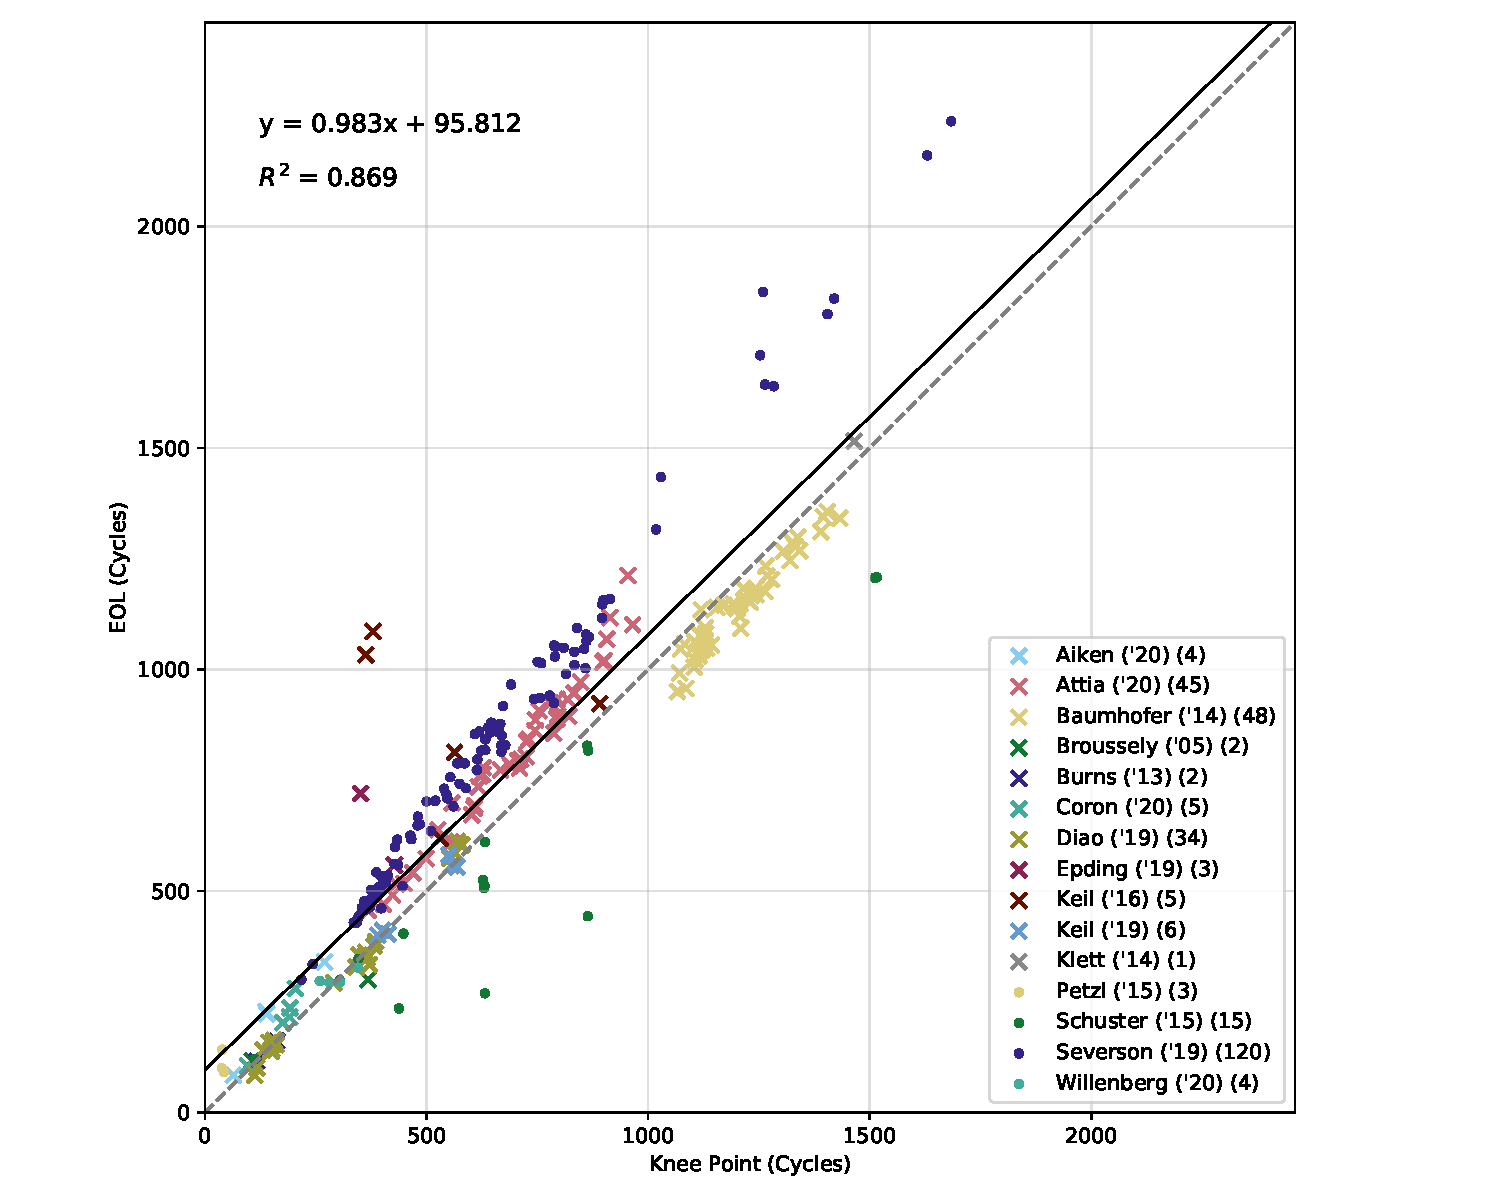
\includegraphics[scale=0.70]{final_figures/AcrossDatasetsknee-to-EOL}
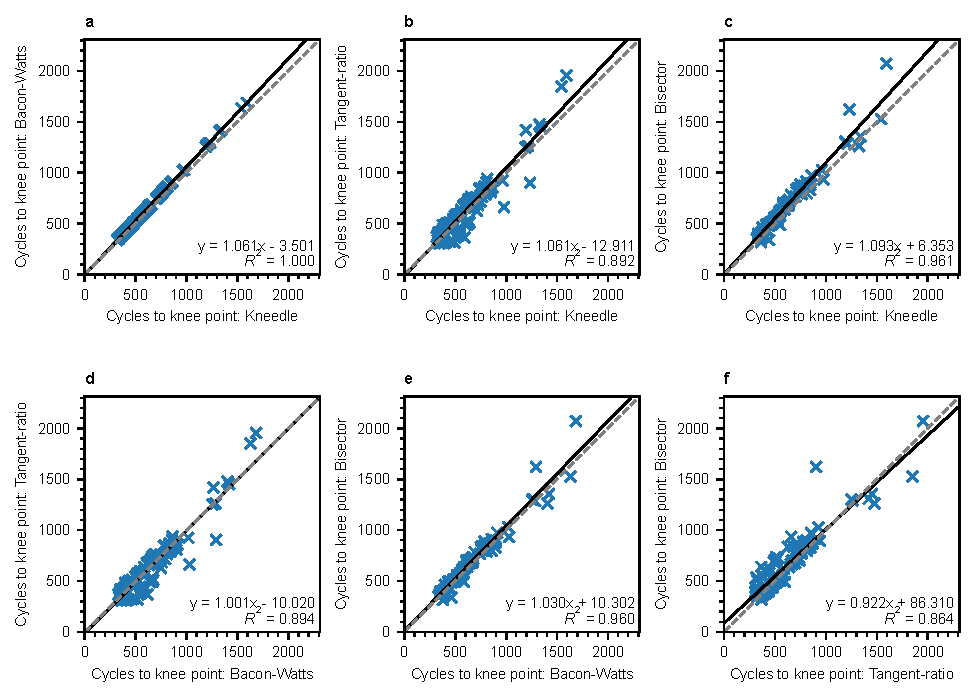
\includegraphics[scale=1.0]{final_figures/severson_knee_compare_all_algorithms.pdf}
%   \caption{Linear regression of knee-point to EOL point}
% \end{subfigure}%
\caption{
Linear regressions comparing various knee point estimation algorithms for the capacity curves of the Severson et al. \cite{severson_data-driven_2019} dataset (except the quantile regression method\cite{zhang_identifying_2020}). We mention that the true knee point has no ``ground truth''.
The results from the Kneedle\cite{satopaa_finding_2011} and Bacon-Watts\cite{fermin-cueto_identification_2020} methods are highly correlated with each other ($R^2\approx 1$). The bisector\cite{greenbank_automated_2021} is also highly correlated with these two methods ($R^2\approx 0.96$). The tangent-ratio method \cite{diao_algorithm_2019} has the poorest correlation with the others.
}.
\label{fig:severson_knee_compare_all_algorithms}
\end{figure}

\begin{figure}[ht]
\centering
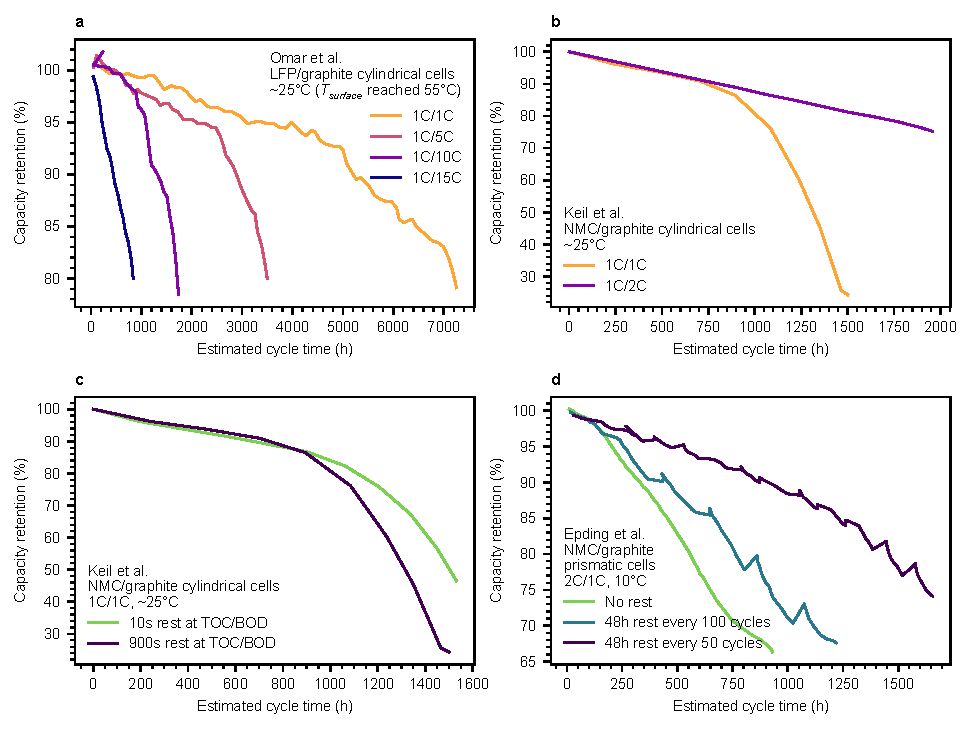
\includegraphics[scale = 1.0]{final_figures/discharge_rate_rest_time.pdf}
\caption{Mixed effects of discharge rate and rest time on knee onset, depending on the testing conditions.
Data replotted from Figure 20 with a time-based $x$ axis (estimated from C rates).
Raw data from the corresponding studies were not available, so the cycle times were estimated from the given C rates and rest times.
While the trends in discharge rate and rest time influence on knee onset are largely the same as in the cycle-based figure (Figure 20), the change from Figure 20c to Figure \ref{fig:discharge-rest_time}c suggests that much of the reason that longer rest times at top-of-charge and bottom-of-discharge decrease cycle life (at least in this study) is calendar aging, not greater degradation at the voltage extremes.
Thus, the use of a cycle-based $x$ axis may obscure calendar aging phenomena. 
(a) Higher discharge rate can accelerate knee onset. Adapted from Figure 8 of Omar et al.\cite{omar_lithium_2014}
Note that while the environmental test temperature was $\sim$25\degree C, the temperature at the surface reached as high as 55\degree C for the high rate discharge tests.
(b) Lower discharge rate can accelerate knee onset. Adapted from Figure 2a of Keil et al.\cite{keil_linear_2019} (c) Longer rest time can accelerate knee onset. Adapted from  Figure 2a of Keil et al.\cite{keil_linear_2019} (d) Shorter rest time can accelerate knee onset. Adapted from Figure 1a of Epding et al.\cite{epding_investigation_2019}.}
\label{fig:discharge-rest_time}
\end{figure}

\begin{figure}[ht]
\centering
% \begin{subfigure}{.5\textwidth}
%   \centering
% 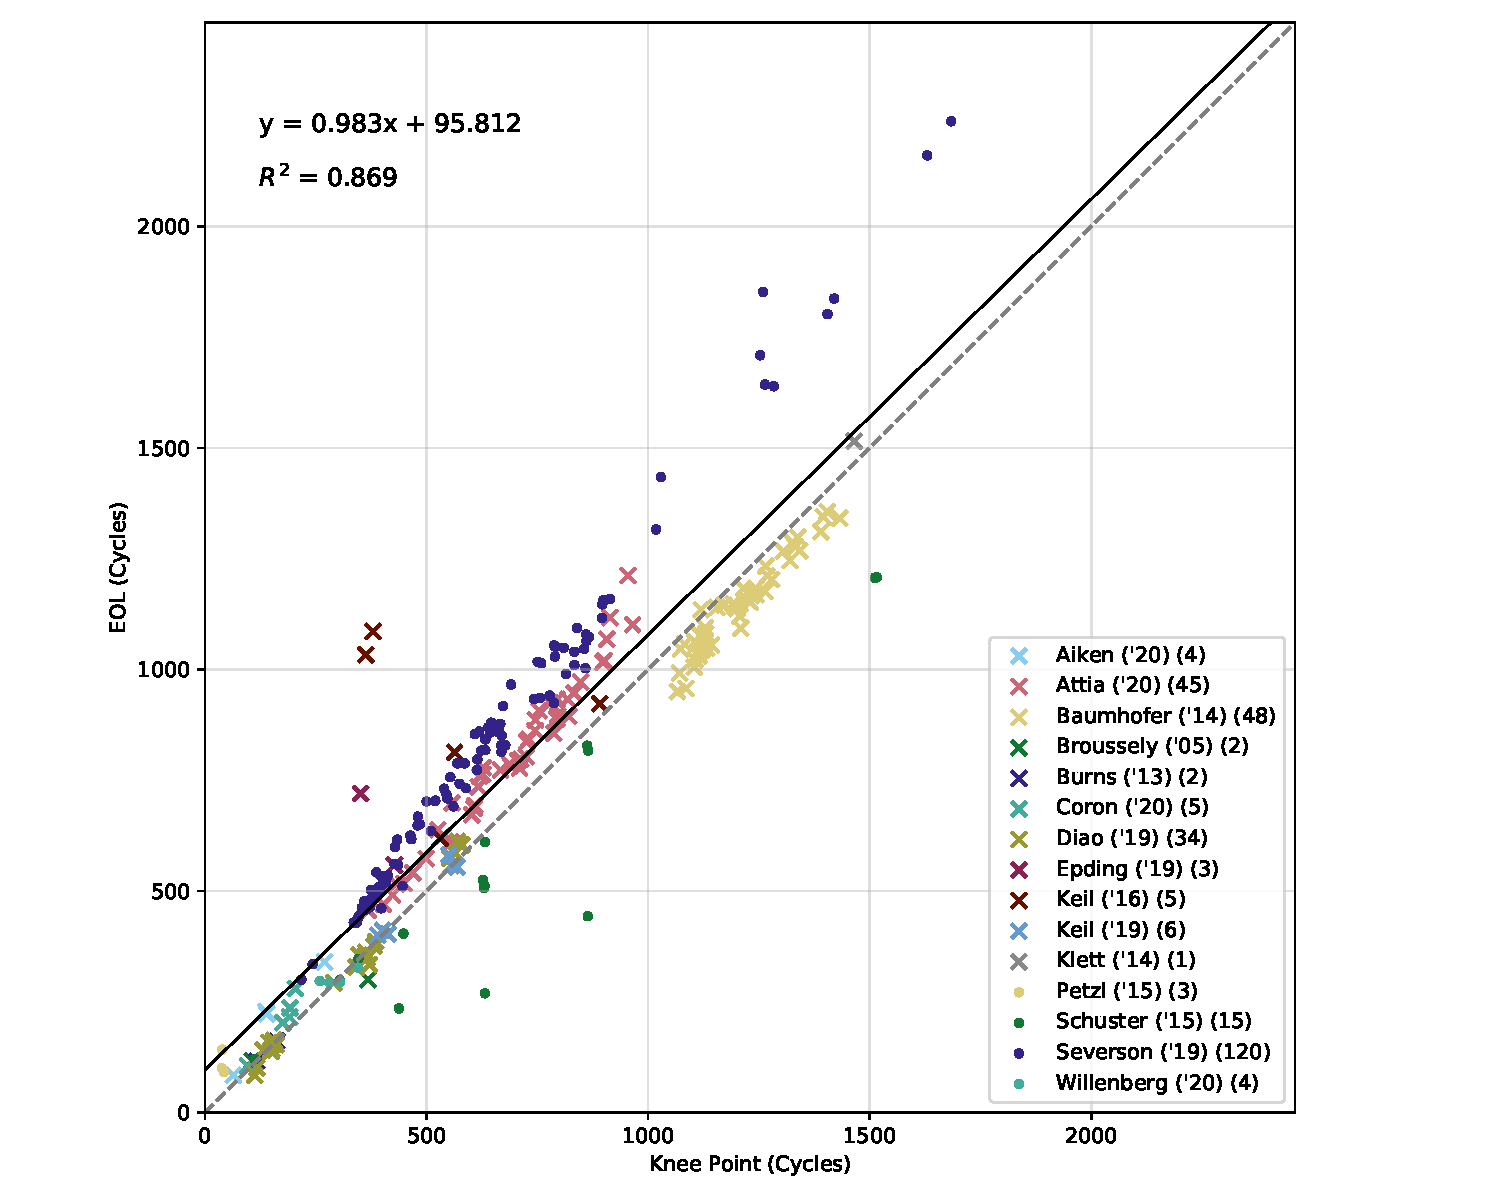
\includegraphics[scale=0.70]{final_figures/AcrossDatasetsknee-to-EOL}
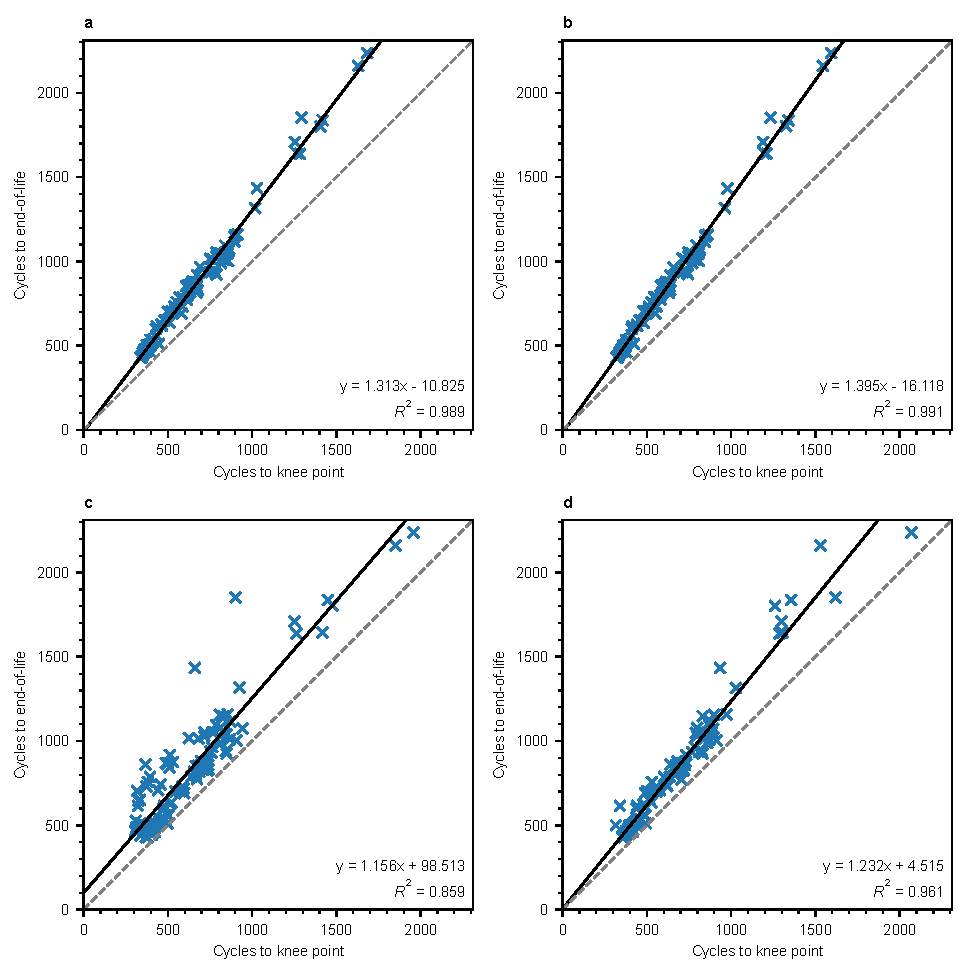
\includegraphics[scale=1.0]{final_figures/severson_knee_eol_all_algorithms.pdf}
%   \caption{Linear regression of knee-point to EOL point}
% \end{subfigure}%
\caption{Linear relationship between identified knees and end-of-life (EOL) per knee identification algorithm over the Severson et al. \cite{severson_data-driven_2019} dataset.
(a) Bacon-Watts\cite{fermin-cueto_identification_2020}{},
(b) Kneedle\cite{satopaa_finding_2011}{},
(c) Tangent-ratio\cite{diao_algorithm_2019}{},
(d) Bisector\cite{greenbank_automated_2021}{}.
We mention that there is no ``ground truth'' for the true knee. For the Bacon-Watts and Kneedle identified knees, the linear regression holds with a goodness-of-fit of $R^2\approx 99\%$ (and reduced variance between fit and residuals). With this metric, close by is the bisector\cite{greenbank_automated_2021} with a correlation of $R^2\approx 0.96$. The tangent-ratio\cite{diao_algorithm_2019} identified knees show a higher fit-to-residuals variability ($R^2\approx 0.86$).}.
\label{fig:severson_knee_eol_all_algorithms}
\end{figure}

% \gbox{refer to Yulia's table "SI-EXP Table"// Table \ref{table:experimental_summary}},

% generated via https://www.latex-tables.com
\newgeometry{margin=2.5cm}
\begin{landscape}
\begin{table}[p]
\caption{Summary of references used to generate Figure 22 in the main manuscript.
The data was obtained extracted via direct access to the corresponding databases when possible \cite{baumhofer_production_2014,diao_accelerated_2019,severson_data-driven_2019,willenberg_high-precision_2020,attia_closed-loop_2020} or via \textit{WebPlotDigitizer}\cite{Rohatgi2021}.}
\label{table:experimental_summary_DATASOURCES}
\scalebox{0.75}{\begin{tabular}{|l|l|c|l|} 
\hline
\textbf{Reference}     & \textbf{Cell Description}                                                                                                          & \textbf{Number of cells} & \textbf{Capacity curve references}                                                                                                                                                                                                                                                                                                                                                                                    \\ 
\hline
Aiken et al.\cite{aiken_accelerated_2020} 2020      & Lab-made pouch NMC/Gr                                                                                                              & 4                        & \begin{tabular}[c]{@{}l@{}}Fig 3d 0.8M, 1.2M;\\ Fig 10a: \`{}red circle' and \`{}blue circle'\end{tabular}                                                                                                                                                                                                                                                                                                            \\ 
\hline
Baumh\"{o}fer et al.\cite{baumhofer_production_2014} 2014  & Sanyo UR18650E NMC/Gr                                                                                                              & 48                       & Database access                                                                                                                                                                                                                                                                                                                                                                                                       \\ 
\hline
Broussely et al.\cite{broussely_main_2005} 2005  & Saft VLE NCA/Gr                                                                                                                    & 2                        & Fig 2 red and green                                                                                                                                                                                                                                                                                                                                                                                                   \\ 
\hline
Burns et al.\cite{burns_-situ_2015} 2015      & Panasonic 18650 NCA/Gr                                                                                                             & 2                        & Fig1b circles and squares                                                                                                                                                                                                                                                                                                                                                                                             \\ 
\hline
Coron et al.\cite{coron_impact_2020} 2020      & \begin{tabular}[c]{@{}l@{}}Commercial 18650 NMC+LMO/Gr\\ Commercial 18650 NMC/Gr\end{tabular}                                      & 5                        & \begin{tabular}[c]{@{}l@{}}Fig 1c: \`{}red crosses', \`{}red squares',\\ \`{}blue crosses', \`{}blue squares' and \`{}blue circles'\end{tabular}                                                                                                                                                                                                                                                                      \\ 
\hline
Diao et al.\cite{diao_accelerated_2019} 2019       & Pouch LCO/Gr                                                                                                                       & 34                       & Database access                                                                                                                                                                                                                                                                                                                                                                                                       \\ 
\hline
Epding et al.\cite{epding_investigation_2019} 2019     & Commercial prismatic NMC/Gr                                                                                                        & 3                        & Fig 1a black and green; Fig 7a black cell 2                                                                                                                                                                                                                                                                                                                                                                           \\ 
\hline
Keil et al.\cite{keil_charging_2016} 2016       & \begin{tabular}[c]{@{}l@{}}a) Sanyo UR18650SA LMO+NMC/Gr\\ b) Sony US18650VT1 LMO+LCO/Gr\\ c) A123 APR18650M1A LFP/Gr\end{tabular} & 5                        & \begin{tabular}[c]{@{}l@{}}Fig 8c 3A CCCV +50mV (C); Fig 10a 1A CCCV (A);\\ Fig 10a 1A CCCV (A); Fig 10b 3A CCCV (B);\\ Fig 10c 5A CCCV (C)\end{tabular}                                                                                                                                                                                                                                                              \\ 
\hline
Keil et al.\cite{keil_linear_2019} 2019       & Cylindrical NMC/Gr                                                                                                                 & 6                        & \begin{tabular}[c]{@{}l@{}}Fig 2a procedure 1 and 2; Fig 8a procedure 1 100 SOC; \\Fig 8a procedure 1 0 SOC; Fig 8a procedure 2 100 SOC; \\Fig 8a procedure 2 0 SOC\end{tabular}                                                                                                                                                                                                                                      \\ 
\hline
Klett et al.\cite{klett_non-uniform_2014} 2014      & Commercial 26650 LFP/Gr                                                                                                            & 1                        & Figure 2a CCC                                                                                                                                                                                                                                                                                                                                                                                                         \\ 
\hline
Petzl et al.\cite{petzl_lithium_2015} 2015      & Commercial 26650 LFP/Gr                                                                                                            & 3                        & Fig 1a blue, red, black                                                                                                                                                                                                                                                                                                                                                                                               \\ 
\hline
Schuster et al.\cite{schuster_nonlinear_2015} 2015   & E-One Moli Energy IHR18650A NMC/Gr                                                                                                 & 15                       & \begin{tabular}[c]{@{}l@{}}Fig 1a; Fig 4a 1.30V (CCCV) (A); Fig 4a 1.20V (CCCV) (A); \\ Fig 4a 1.20V (CC) (A); Fig 4a 0.94V (CC) (A); \\ Fig 6a 0.5C/0.5C (A); Fig 6a 1.0C/0.5C (A); Fig 6a 0.5C/1.0C (A); \\ Fig 9 1.20 V (CC); Fig 9 1.20 V (CCCV); Fig 9 1.20 V (2CCCV); \\ Fig 10a 35 C(deltaV down) (A); Fig 10a 35 C(deltaV up) (A); \\ Fig 10a 50 C(deltaV up) (A); Fig 10a 25 C(deltaV up) (A);\end{tabular}  \\ 
\hline
Severson et al.\cite{severson_data-driven_2019} 2019   & A123 APR18650M1A LFP/Gr                                                                                                            & 120                      & Database access                                                                                                                                                                                                                                                                                                                                                                                                       \\ 
\hline
Willenberg et al.\cite{willenberg_high-precision_2020} 2020 & Samsung INR18650 35E NCA/Gr+Si                                                                                                     & 4                        & Database access                                                                                                                                                                                                                                                                                                                                                                                                       \\
\hline
\end{tabular}
}
\end{table}

\end{landscape}
\restoregeometry


% \bibliographystyle{myIEEEtran}
\bibliography{refs_zotero}

\end{document}